\documentclass{beamer}
\usepackage{beamerthemesplit}
\usepackage{color,xcolor,ucs}
\usetheme{Warsaw}
\usepackage{graphicx}
\usepackage{ulem}
\usepackage{tikz}
\usetikzlibrary{shapes,arrows}
\usepackage{subcaption}
\usepackage{algorithm,algorithmic}
\usepackage{natbib}
\usepackage{cancel}
% include.tex
\newcommand{\Bernoulli}[1]{\text{Bernoulli} \left( #1 \right)}
\newcommand{\mydigamma}[1]{\psi \left( #1 \right)}
%\newcommand{\diag}[1]{\text{diag}\left( #1 \right)}
\newcommand{\tr}[1]{\text{tr}\left( #1 \right)}
\newcommand{\Poisson}[1]{\text{Poisson} \left( #1 \right)}
\def \half {\frac{1}{2}}
\def \R {\mathbb{R}}
\def \vbeta {\vec{\beta}}
\def \vy {\vec{y}}
\def \vmu {\vec{\mu}}
\def \vmuqbeta {\vmu_{q(\vbeta)}}
\def \vmubeta {\vmu_{\vbeta}}
\def \Sigmaqbeta {\Sigma_{q(\vbeta)}}
\def \Sigmabeta {\Sigma_{\vbeta}}
\def \va {\vec{a}}
\def \vtheta {\vec{\theta}}
\def \mX {\vec{X}}

\def\ds{{\displaystyle}}

\def\diag{{\mbox{diag}}}


\usepackage{latexsym,amssymb,amsmath,amsfonts}
%\usepackage{tabularx}
\usepackage{theorem}
\usepackage{verbatim,array,multicol,palatino}
\usepackage{graphicx}
\usepackage{graphics}
\usepackage{fancyhdr}
\usepackage{algorithm,algorithmic}
\usepackage{url}
%\usepackage[all]{xy}



\def\approxdist{\stackrel{{\tiny \mbox{approx.}}}{\sim}}
\def\smhalf{\textstyle{\frac{1}{2}}}
\def\vxnew{\vx_{\mbox{{\tiny new}}}}
\def\bib{\vskip12pt\par\noindent\hangindent=1 true cm\hangafter=1}
\def\jump{\vskip3mm\noindent}
\def\etal{{\em et al.}}
\def\etahat{{\widehat\eta}}
\def\thick#1{\hbox{\rlap{$#1$}\kern0.25pt\rlap{$#1$}\kern0.25pt$#1$}}
\def\smbbeta{{\thick{\scriptstyle{\beta}}}}
\def\smbtheta{{\thick{\scriptstyle{\theta}}}}
\def\smbu{{\thick{\scriptstyle{\rm u}}}}
\def\smbzero{{\thick{\scriptstyle{0}}}}
\def\boxit#1{\begin{center}\fbox{#1}\end{center}}
\def\lboxit#1{\vbox{\hrule\hbox{\vrule\kern6pt
      \vbox{\kern6pt#1\kern6pt}\kern6pt\vrule}\hrule}}
\def\thickboxit#1{\vbox{{\hrule height 1mm}\hbox{{\vrule width 1mm}\kern6pt
          \vbox{\kern6pt#1\kern6pt}\kern6pt{\vrule width 1mm}}
               {\hrule height 1mm}}}


%\sloppy
%\usepackage{geometry}
%\geometry{verbose,a4paper,tmargin=20mm,bmargin=20mm,lmargin=40mm,rmargin=20mm}


%%%%%%%%%%%%%%%%%%%%%%%%%%%%%%%%%%%%%%%%%%%%%%%%%%%%%%%%%%%%%%%%%%%%%%%%%%%%%%%%
%
% Some convenience definitions
%
% \bf      -> vector
% \sf      -> matrix
% \mathcal -> sets or statistical
% \mathbb  -> fields or statistical
%
%%%%%%%%%%%%%%%%%%%%%%%%%%%%%%%%%%%%%%%%%%%%%%%%%%%%%%%%%%%%%%%%%%%%%%%%%%%%%%%%

% Sets or statistical values
\def\sI{{\mathcal I}}                            % Current Index set
\def\sJ{{\mathcal J}}                            % Select Index set
\def\sL{{\mathcal L}}                            % Likelihood
\def\sl{{\ell}}                                  % Log-likelihood
\def\sN{{\mathcal N}}                            
\def\sS{{\mathcal S}}                            
\def\sP{{\mathcal P}}                            
\def\sQ{{\mathcal Q}}                            
\def\sB{{\mathcal B}}                            
\def\sD{{\mathcal D}}                            
\def\sT{{\mathcal T}}
\def\sE{{\mathcal E}}                            
\def\sF{{\mathcal F}}                            
\def\sC{{\mathcal C}}                            
\def\sO{{\mathcal O}}                            
\def\sH{{\mathcal H}} 
\def\sR{{\mathcal R}}                            
\def\sJ{{\mathcal J}}                            
\def\sCP{{\mathcal CP}}                            
\def\sX{{\mathcal X}}                            
\def\sA{{\mathcal A}} 
\def\sZ{{\mathcal Z}}                            
\def\sM{{\mathcal M}}                            
\def\sK{{\mathcal K}}     
\def\sG{{\mathcal G}}                         
\def\sY{{\mathcal Y}}                         
\def\sU{{\mathcal U}}  


\def\sIG{{\mathcal IG}}                            


\def\cD{{\sf D}}
\def\cH{{\sf H}}
\def\cI{{\sf I}}

% Vectors
\def\vectorfontone{\bf}
\def\vectorfonttwo{\boldsymbol}
\def\va{{\vectorfontone a}}                      %
\def\vb{{\vectorfontone b}}                      %
\def\vc{{\vectorfontone c}}                      %
\def\vd{{\vectorfontone d}}                      %
\def\ve{{\vectorfontone e}}                      %
\def\vf{{\vectorfontone f}}                      %
\def\vg{{\vectorfontone g}}                      %
\def\vh{{\vectorfontone h}}                      %
\def\vi{{\vectorfontone i}}                      %
\def\vj{{\vectorfontone j}}                      %
\def\vk{{\vectorfontone k}}                      %
\def\vl{{\vectorfontone l}}                      %
\def\vm{{\vectorfontone m}}                      % number of basis functions
\def\vn{{\vectorfontone n}}                      % number of training samples
\def\vo{{\vectorfontone o}}                      %
\def\vp{{\vectorfontone p}}                      % number of unpenalized coefficients
\def\vq{{\vectorfontone q}}                      % number of penalized coefficients
\def\vr{{\vectorfontone r}}                      %
\def\vs{{\vectorfontone s}}                      %
\def\vt{{\vectorfontone t}}                      %
\def\vu{{\vectorfontone u}}                      % Penalized coefficients
\def\vv{{\vectorfontone v}}                      %
\def\vw{{\vectorfontone w}}                      %
\def\vx{{\vectorfontone x}}                      % Covariates/Predictors
\def\vy{{\vectorfontone y}}                      % Targets/Labels
\def\vz{{\vectorfontone z}}                      %

\def\vone{{\vectorfontone 1}}
\def\vzero{{\vectorfontone 0}}

\def\valpha{{\vectorfonttwo \alpha}}             %
\def\vbeta{{\vectorfonttwo \beta}}               % Unpenalized coefficients
\def\vgamma{{\vectorfonttwo \gamma}}             %
\def\vdelta{{\vectorfonttwo \delta}}             %
\def\vepsilon{{\vectorfonttwo \epsilon}}         %
\def\vvarepsilon{{\vectorfonttwo \varepsilon}}   % Vector of errors
\def\vzeta{{\vectorfonttwo \zeta}}               %
\def\veta{{\vectorfonttwo \eta}}                 % Vector of natural parameters
\def\vtheta{{\vectorfonttwo \theta}}             % Vector of combined coefficients
\def\vvartheta{{\vectorfonttwo \vartheta}}       %
\def\viota{{\vectorfonttwo \iota}}               %
\def\vkappa{{\vectorfonttwo \kappa}}             %
\def\vlambda{{\vectorfonttwo \lambda}}           % Vector of smoothing parameters
\def\vmu{{\vectorfonttwo \mu}}                   % Vector of means
\def\vnu{{\vectorfonttwo \nu}}                   %
\def\vxi{{\vectorfonttwo \xi}}                   %
\def\vpi{{\vectorfonttwo \pi}}                   %
\def\vvarpi{{\vectorfonttwo \varpi}}             %
\def\vrho{{\vectorfonttwo \rho}}                 %
\def\vvarrho{{\vectorfonttwo \varrho}}           %
\def\vsigma{{\vectorfonttwo \sigma}}             %
\def\vvarsigma{{\vectorfonttwo \varsigma}}       %
\def\vtau{{\vectorfonttwo \tau}}                 %
\def\vupsilon{{\vectorfonttwo \upsilon}}         %
\def\vphi{{\vectorfonttwo \phi}}                 %
\def\vvarphi{{\vectorfonttwo \varphi}}           %
\def\vchi{{\vectorfonttwo \chi}}                 %
\def\vpsi{{\vectorfonttwo \psi}}                 %
\def\vomega{{\vectorfonttwo \omega}}             %


% Matrices
%\def\matrixfontone{\sf}
%\def\matrixfonttwo{\sf}
\def\matrixfontone{\bf}
\def\matrixfonttwo{\boldsymbol}
\def\mA{{\matrixfontone A}}                      %
\def\mB{{\matrixfontone B}}                      %
\def\mC{{\matrixfontone C}}                      % Combined Design Matrix
\def\mD{{\matrixfontone D}}                      % Penalty Matrix for \vu_J
\def\mE{{\matrixfontone E}}                      %
\def\mF{{\matrixfontone F}}                      %
\def\mG{{\matrixfontone G}}                      % Penalty Matrix for \vu
\def\mH{{\matrixfontone H}}                      %
\def\mI{{\matrixfontone I}}                      % Identity Matrix
\def\mJ{{\matrixfontone J}}                      %
\def\mK{{\matrixfontone K}}                      %
\def\mL{{\matrixfontone L}}                      % Lower bound
\def\mM{{\matrixfontone M}}                      %
\def\mN{{\matrixfontone N}}                      %
\def\mO{{\matrixfontone O}}                      %
\def\mP{{\matrixfontone P}}                      %
\def\mQ{{\matrixfontone Q}}                      %
\def\mR{{\matrixfontone R}}                      %
\def\mS{{\matrixfontone S}}                      %
\def\mT{{\matrixfontone T}}                      %
\def\mU{{\matrixfontone U}}                      % Upper bound
\def\mV{{\matrixfontone V}}                      %
\def\mW{{\matrixfontone W}}                      % Variance Matrix i.e. diag(b'')
\def\mX{{\matrixfontone X}}                      % Unpenalized Design Matrix/Nullspace Matrix
\def\mY{{\matrixfontone Y}}                      %
\def\mZ{{\matrixfontone Z}}                      % Penalized Design Matrix/Kernel Space Matrix

\def\mGamma{{\matrixfonttwo \Gamma}}             %
\def\mDelta{{\matrixfonttwo \Delta}}             %
\def\mTheta{{\matrixfonttwo \Theta}}             %
\def\mLambda{{\matrixfonttwo \Lambda}}           % Penalty Matrix for \vnu
\def\mXi{{\matrixfonttwo \Xi}}                   %
\def\mPi{{\matrixfonttwo \Pi}}                   %
\def\mSigma{{\matrixfonttwo \Sigma}}             %
\def\mUpsilon{{\matrixfonttwo \Upsilon}}         %
\def\mPhi{{\matrixfonttwo \Phi}}                 %
\def\mOmega{{\matrixfonttwo \Omega}}             %
\def\mPsi{{\matrixfonttwo \Psi}}                 %

\def\mone{{\matrixfontone 1}}
\def\mzero{{\matrixfontone 0}}

% Fields or Statistical
\def\bE{{\mathbb E}}                             % Expectation
\def\bP{{\mathbb P}}                             % Probability
\def\bR{{\mathbb R}}                             % Reals
\def\bI{{\mathbb I}}                             % Reals
\def\bV{{\mathbb V}}                             % Reals

\def\vX{{\vectorfontone X}}                      % Targets/Labels
\def\vY{{\vectorfontone Y}}                      % Targets/Labels
\def\vZ{{\vectorfontone Z}}                      %

% Other
\def\etal{{\em et al.}}
\def\ds{\displaystyle}
\def\d{\partial}
\def\diag{\text{diag}}
%\def\span{\text{span}}
\def\blockdiag{\text{blockdiag}}
\def\tr{\text{tr}}
\def\RSS{\text{RSS}}
\def\df{\text{df}}
\def\GCV{\text{GCV}}
\def\AIC{\text{AIC}}
\def\MLC{\text{MLC}}
\def\mAIC{\text{mAIC}}
\def\cAIC{\text{cAIC}}
\def\rank{\text{rank}}
\def\MASE{\text{MASE}}
\def\SMSE{\text{SASE}}
\def\sign{\text{sign}}
\def\card{\text{card}}
\def\notexp{\text{notexp}}
\def\ASE{\text{ASE}}
\def\ML{\text{ML}}
\def\nullity{\text{nullity}}

\def\logexpit{\text{logexpit}}
\def\logit{\mbox{logit}}
\def\dg{\mbox{dg}}

\def\Bern{\mbox{Bernoulli}}
\def\sBernoulli{\mbox{Bernoulli}}
\def\sGamma{\mbox{Gamma}}
\def\sInvN{\mbox{Inv}\sN}
\def\sNegBin{\sN\sB}

\def\dGamma{\mbox{Gamma}}
\def\dInvGam{\mbox{Inv}\Gamma}

\def\Cov{\mbox{Cov}}
\def\Mgf{\mbox{Mgf}}

\def\mis{{mis}} 
\def\obs{{obs}}

\def\argmax{\operatornamewithlimits{\text{argmax}}}
\def\argmin{\operatornamewithlimits{\text{argmin}}}
\def\argsup{\operatornamewithlimits{\text{argsup}}}
\def\arginf{\operatornamewithlimits{\text{arginf}}}


\def\minimize{\operatornamewithlimits{\text{minimize}}}
\def\maximize{\operatornamewithlimits{\text{maximize}}}
\def\suchthat{\text{such that}}


\def\relstack#1#2{\mathop{#1}\limits_{#2}}
\def\sfrac#1#2{{\textstyle{\frac{#1}{#2}}}}


\def\comment#1{
\vspace{0.5cm}
\noindent \begin{tabular}{|p{14cm}|}  
\hline #1 \\ 
\hline 
\end{tabular}
\vspace{0.5cm}
}


\def\mytext#1{\begin{tabular}{p{13cm}}#1\end{tabular}}
\def\mytextB#1{\begin{tabular}{p{7.5cm}}#1\end{tabular}}
\def\mytextC#1{\begin{tabular}{p{12cm}}#1\end{tabular}}

\def\jump{\vskip3mm\noindent}

\def\KL{\text{KL}}
\def\N{\text{N}}
\def\Var{\text{Var}}

\def \E {\mathbb{E}}
\def \BigO {\text{O}}
\def \IG {\text{IG}}
\def \Beta {\text{Beta}}



\usefonttheme{serif}

\title{Exact expressions for parameter posteriors in Bayesian linear model selection}
\author{Mark Greenaway, Dr John Ormerod}

\mode<presentation>
{ \usetheme{boxes} }


\begin{document}
% 1. Front slide
\begin{frame}
	\titlepage
	% Details about myself here?
\end{frame}

\note{Hello everyone, I'm Mark Greenaway and I'm a PhD candidate from the University of Sydney.
			I'll be presenting on exact expressions for parameter posteriors
			in Bayesian linear model selection. This is joint work with Dr John Ormerod.}
			
% Only have ten minutes
% Introduce problem
\begin{frame}
	\frametitle{Posterior parameters in Bayesian linear model selection}
	\begin{itemize}
		\item Motivation: The problem of selecting linear models is well-studied, in both the frequentist and Bayesian contexts.
		
		\item A lot of work has been done on specifying parameter priors for Bayesian model selection.
		
		\item Less work has been done on the parameter posteriors. 
		%Here we explore this area in our
		%			research.
					
		\item Typical approaches to finding these posterior distributions would require slow Monte Carlo methods, or crude
		normal approximations.
					
		\item We derive several new exact closed form expressions for the parameter posteriors for a popular choice of priors for linear models.
		
		\item These expressions are in terms of special functions and  are numerically well-behaved, accurate, and fast to evaluate.
	\end{itemize}
\end{frame}

\note{%Linear model selection is a well-studied problem. A lot of work has been done on studying parameter priors
			%for model selection. The parameter posteriors are less well-studied, so we chose to explore this area in
			%our research. We derive several new exact closed form expressions for the posterior parameters using
			%special functions. These expressions are numerically well-behaved, and can be evaluated with widely 
			%available	libraries.

			People have looked at particular combinations of models and priors, calculating the marginal
			likelihoods.
			The next step in the process would be to look at the posteriors of individual parameters.
			We derive several new exact closed form expressions for the posterior parameters using
			special functions. These expressions are numerically well-behaved, and can be evaluated with widely 
			available	libraries.
			We also want to look at the numerical properties of these expressions, as we want them to be numerically
			stable and easy to evaluate.}

 

% Introduce model
\begin{frame}
	\frametitle{Model selection using $g$}
	\begin{itemize}
		\item 	 Let $\vy$ be the vector of responses of length $n$, and $\mX$ be the $n \times p$ covariate matrix with linear model		
			\begin{align*}
	\vy | \alpha, \vbeta, \sigma^2 \sim \N(\vone \alpha + \mX \vbeta, \sigma^2 \mI) 
	\end{align*}	
		
		\item We adopt the prior structure on $\vbeta$ called a $g$-prior on $\vbeta$, introduced in
		\cite{Zellner1986}.
		\begin{align*}
			\alpha \quad & \propto \quad 1, \\
			\vbeta | \sigma^2, g \quad & \sim \quad \N_p(\vzero, g \sigma^2 (\mX^\top \mX)^{-1}),                     \\
			p(\sigma^2)          \quad & = \quad (\sigma^2)^{-1} \I(\sigma^2 > 0), \text{ and }                    \\
			p(g)                 \quad & = \quad \text{unspecified for now}.
		\end{align*}
		% FIXME: Can you rewrite this so that it's more clearly expressed?
		% shrinkage of prior controlled by g, how diffuse it is
		\item $g$ controls the shrinkage of $\vbeta$: if $g$ is high there is not much shrinkage,
					and if $g$ is low there is a lot of shrinkage.
		% that controls the mixing between the null and full models.
		% \item If $g$ is $0$, we
		% choose the null model. If $g$ is $\infty$ we choose $\hat{\vbeta}$.
	\end{itemize}
\end{frame}

\note{We adopt a linear model with the following structure.
			This structure is chosen with great care so that the the parameters can be integrated out analytically.
			We introduce a parameter $g$ which controls the shrinkage: if $g$ is high there is not much shrinkage,
			and if $g$ is low there is a lot of shrinkage.}

% Discuss Bartlett's and Information Paradox
%\begin{frame}
%	\frametitle{How should we choose $g$?}
%	There are a few approaches we could take.
%	\begin{itemize}
%		\item We could simply let $g \to \infty$.
%		\item \cite{Liang2008} discussed that\\
%		$p(\vgamma = \vzero | \vy) \to 1$ as $g \to \infty$ (Bartlett's paradox).
%		\item We could make a fixed choice of $g$. \\
%		\item \cite{Liang2008} discussed that \\
%					$p(\vgamma = \vgamma^* | \vy) \cancel{\to} 1$ as $R_\vgamma^2 \to 1$, \\
%					where $\vgamma^*$ is the true model (Information Paradox)
%		\item We could choose $g$ adaptively, using Empirical Bayes
%		\item \cite{Liang2008} showed that this was not model selection consistent if the true model is the null
%					model.
%		\item So we need another approach.
%	\end{itemize}
%\end{frame}

\note{So how should we choose $g$?
			We could let $g$ go to infinity.
			If we have $g$ large, we have a diffuse prior on the coefficients. This places a lot of weight on the
			null model, which is an example of Bartlett's Paradox.
			We could make a fixed choice of $g$, but then we don't necessarily select the true model, even if the
			sample size goes to infinity, which is an example of the Information Paradox.
			We could use Empirical Bayes to choose $g$ adaptively, but Liang showed that this was not model selection
			consistent
			So we need another approach.}

% Mixture of g, choice of g prior
\begin{frame}
	\frametitle{We should choose a mixture of $g$}
	\cite{Liang2008} argued that    
	technical issues with the specification of $g$ can {\bf only}
	be avoided by specifying a hyper-prior for $g$.

	A popular choice of prior is
	$$
	p(g) = \frac{g^b (1 + g)^{-(a + b + 2)}}{\text{Beta}(a + 1, b + 1)} \I(g > 0)
	$$
	
	by \cite{Maruyama2011}, where
	$a = -3/4$, and
	$b = (n - p)/2 - a - 2$.	
\end{frame}


\begin{frame}
	\frametitle{Model selection using $p(\vy)$}
	Model selection can be performed by comparing the marginal likelihoods $p(\vy)$ for different models with
	$$
	\begin{array}{rl}
	p(\vy) 
	& \ds = \int p(\vy|\alpha,\vbeta,\sigma^2,g)p(\alpha)p(\vbeta|\sigma^2,g)p(\sigma^2)p(g) d\alpha d\vbeta d\sigma^2 dg
	\\
	& \ds 
	=  K(n)
	\frac{\mbox{Beta}(p/2 + a + 1,b + 1)}{\mbox{Beta}(a+1,b+1)} (1 - R^2)^{-(b + 1)}
	\end{array} 
	$$

	\noindent where $K(n)$ common to all models.
	This is numerically stable to evaluate
	and asymptotically equivalent to using BIC.
\end{frame}

\note{In order to avoid the problems in the previous slide, Liang argued we should put a prior on $g$.
			Several choices of prior for $g$ have been proposed in the literature.
			These all place most of the prior probability on lower values of $g$, adjusting the shrinkage according
			to the sample size and number of covariates in the model.}

\begin{frame}
	\frametitle{Special functions}
	\begin{itemize}
		\item When $|z| < 1$, the hypergeometric function is defined by the power series
					\[
						{}_2 F_1 (a, b; c; z) = \sum_{n=0}^\infty \frac{(a)_n (b)_n}{(c)_n} \frac{z^n}{n!}
					\]
					where
					$(q)_n = \begin{cases}
						1 & n = 0 \\
						q (q + 1) \ldots (q + n - 1) & n > 0
					\end{cases}$
		\item The confluent hypergeometric function is defined by the power series
					\[
						{}_1 F_1 (a; b; z) = \sum_{n=0}^\infty \frac{(a)_n}{(b)_n} \frac{z^n}{n!}
					\]
		\item These functions can be difficult to numerically evaluate in practice, \S 5.14 \cite{Press:2007:NRE:1403886}.
					We must choose our expressions involving ${}_2 F_1$ carefully!
	\end{itemize}
\end{frame}

\note{At this point, I'll introduce the hypergeometric function, which is defined by
			the following power series within the unit circle.
			The confluent hypergeometric function is defined by the somewhat simpler power series at the bottom of
			the slide.
			The series is divergent as $z \to 1$, which is going to come back to haunt us.
			There is no known numerical routine that will evaluate these functions for every possible combination
			of parameters, so they can be difficult to numerically evaluate in practice.}

% Exact posterior distributions using special functions
\begin{frame}
	\frametitle{Exact posterior distributions of $\alpha$, $\sigma^2$ and $g$ using special functions}
	% When deriving exact posterior distributions on the parameters of the model,
	With a Beta-Prime prior on $g$, we were able to derive closed form expressions for the posterior distributions.
	\small
	\begin{align*}
		% p(u | \vy) &= \frac{(1 - R_\vgamma^2)^{b + 1}}{\text{Beta}(b + 1, d + 1)} u^b (1 - u)^d (1 - u R_\vgamma^2)^{-(b + d + 2)} \\
		p(\alpha | \vy) &= \frac{\Gamma(c + \frac{1}{2}) (1 - R^2)^{b + 1}}{\Gamma(c) \sqrt{\pi}} (1 + \alpha^2)^{-n/2}
		{}_2 F_1 \left(d + 1, -\frac{1}{2}; c; \frac{R^2}{1 + \alpha^2}\right) \\
		p(\sigma^2 | \vy) &= \frac{\frac{n}{2} (1 - R^2)^{b + 1}}{\Gamma(c)} (1 - R^2)^{-(c + 1)}
												\exp{\left( -\frac{n}{2 \sigma^2} \right)} {}_1 F_1 \left(b + 1; c; \frac{n R^2}{2 \sigma^2}\right)
												\\
		p(g | \vy) &= \frac{(1 - R^2)^{b + 1} g^b [1 + g (1 - R^2)]^{-(b + d + 2)}}{\text{Beta}(b + 1, d + 1)}
	\end{align*}
	where
	$a = -3/4$,
	$b = (n - p)/2 - a - 2$,
	$c = (n - 1)/2$, and
	$d = c - b - 2 = p / 2 + a$.
\end{frame}

\note{With a Beta-Prime prior on $g$, we derived exact expressions for the posteriors of $g$, $\alpha$ and
			$\sigma^2$ under the Beta-Prime prior. \\
			$g | \vy$ is a generalised Beta-Prime distribution. \\
			We came up with two expressions for $\alpha | \vy$. I've presented the second of these which is using the 
			Euler identity so that the first two arguments are small in magnitude. This causes the series to converge quickly. This looks complicated, but is actually a fancy $t$-distribution. \\
			$\sigma^2 | \vy$ is pretty close to an Inverse Gamma distribution. \\
			These expressions depend only on $n$, $p_\vgamma$ and $R_\vgamma^2$.}

\begin{frame}
	\frametitle{Exact first and second moments of $\vbeta$}
	% We weren't able to find a closed form expression for $\vbeta | \vy$, but 
	We were able to find closed form
	expressions for the first and second moments of $\vbeta | \vy$.
	\small
	\begin{align*}
		\E[\vbeta | \vy] &= M_1 \widehat{\vbeta} \\
		\Cov[\vbeta | \vy] &= \frac{n}{n - 3} (M_1 - M_2 R^2)(\mX^\top \mX)^{-1} + (M_2 - M_1^2) \widehat{\vbeta} \widehat{\vbeta}^\top
	\end{align*}
	where $\widehat{\vbeta}$ is the MLE for $\vbeta$, 
	\small
	\begin{align*}
		M_1 &= \frac{b + 1}{c} {}_2 F_1 (d + 1, 1; c + 1; R^2) \text{ and } \\
		M_2 &= \frac{(b + 1)(b + 2)}{c(c + 1)} {}_2 F_1 (d + 1, 2; c + 2; R^2).
	\end{align*}
	Note that $M_1$ and $M_2$ approach 1 as $n \to \infty$.
	
	Using the delta method, we were able to get the approximation
	\begin{align*}
		\vbeta | \vy \stackrel{approx}{\sim} t_{n-1} \left[M_1 \vbeta, \left(\frac{n}{n - 1}\right) M_1 (1 - M_1 R^2)(\mX^\top \mX)^{-1}\right].
	\end{align*}
\end{frame}

\note{We weren't able to find a closed form expression for the posterior of $\vbeta$, so instead we focused on
			the first and second moments. The mean and covariance are given in terms of $M_1$ and $M_2$ and these
			can be expressed in terms of the hypergeometric function. \\
			Note that $M_1$ and $M_2$ approach 1 as $n \to \infty$, so the posterior expectation and covariance
			asymptotically approach the maximum likelihood estimates in the limit. \\
			Using the Delta method, we were able to derive  that the posterior distribution of $\vbeta$ is
			approximately $t$-distributed.}

% Say sopmething about the Rao-Blackwellisation?

% Graphs of posterior functions
\begin{frame}
	\frametitle{Comparing exact results to Monte Carlo sampling}
	We checked our results by comparing against Monte Carlo sampling and found that they matched closely.
	\begin{figure}[htp]
		\centering
		\begin{center}$
			\begin{array}{ll}
				% \caption{$u | \vy$}
				% \includegraphics[width=.5\textwidth]{uGivenY.pdf} &
				% \caption{$\sigma^2 | \vy$}
				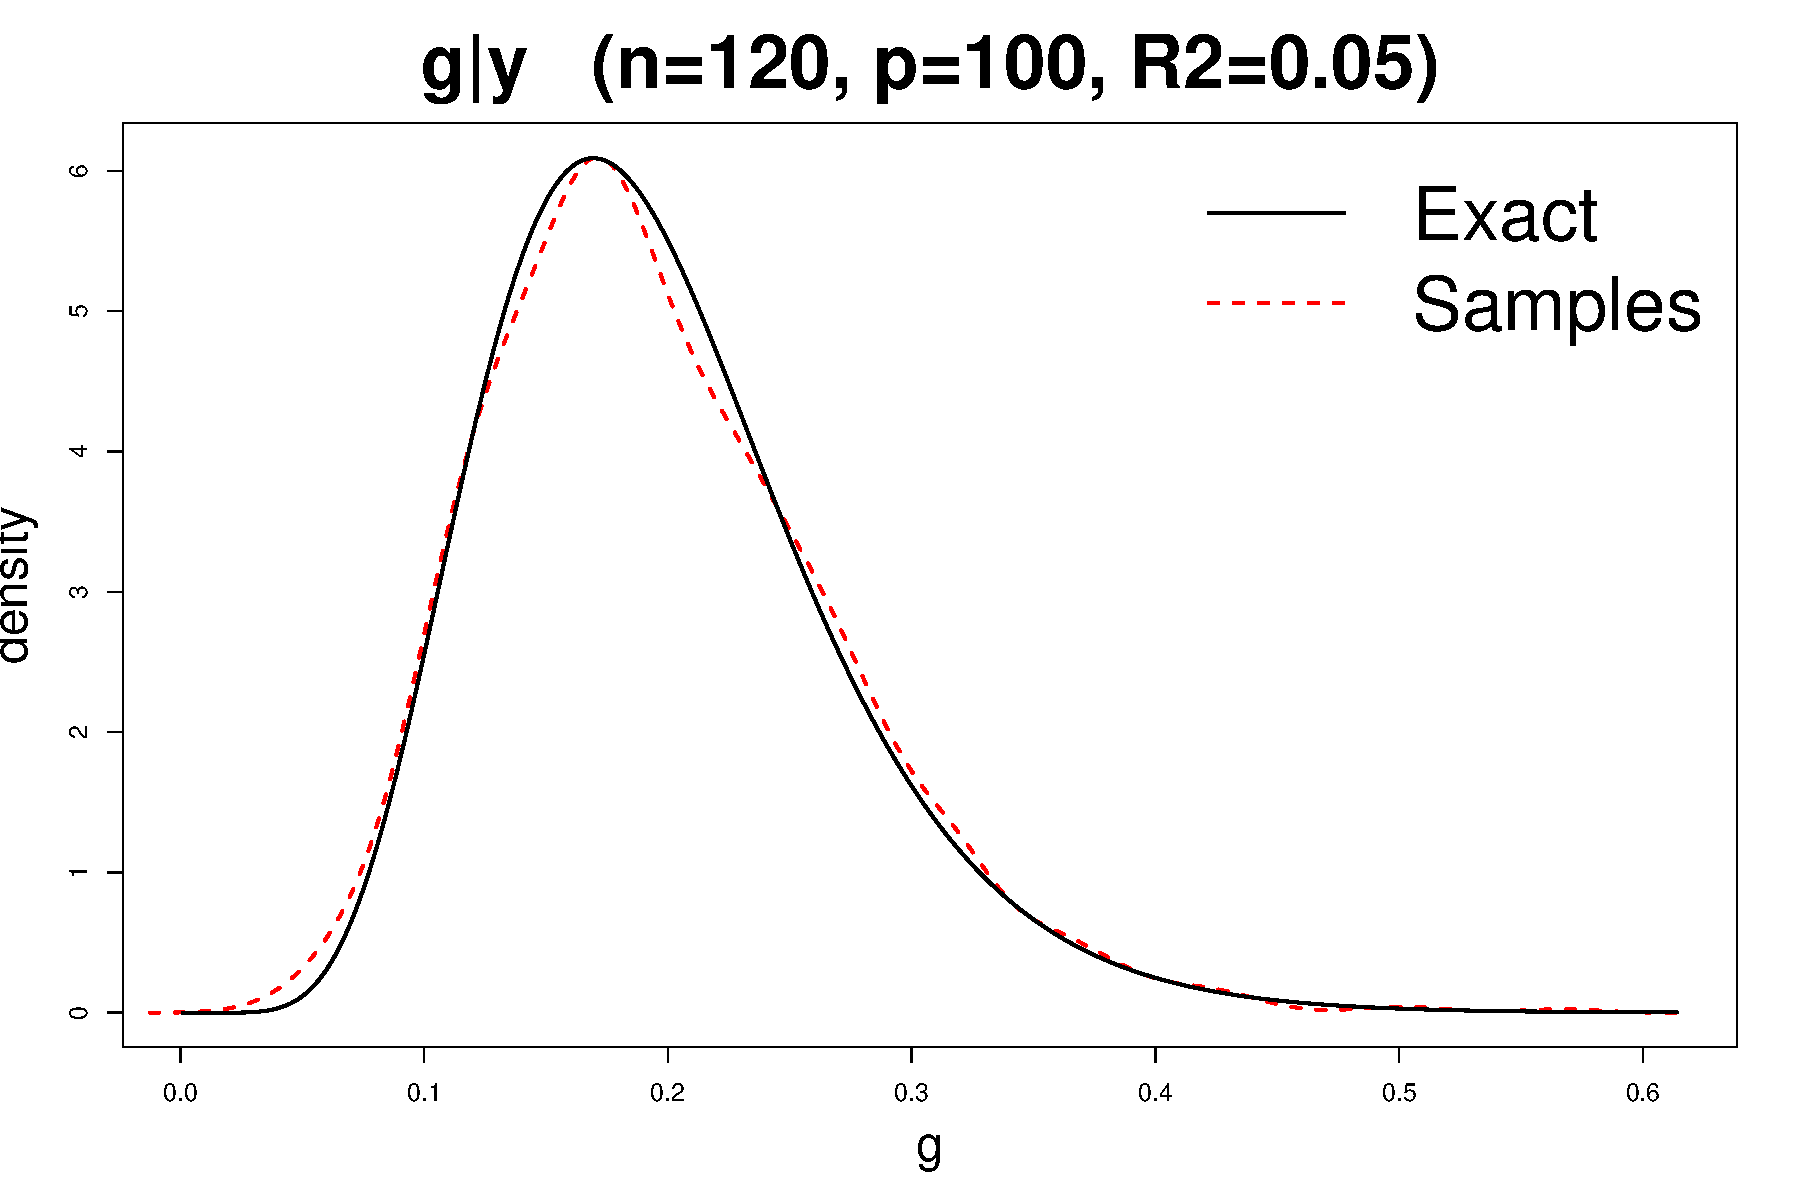
\includegraphics[width=.5\textwidth]{gGivenY.pdf} \\
				% \caption{$g | \vy$}
				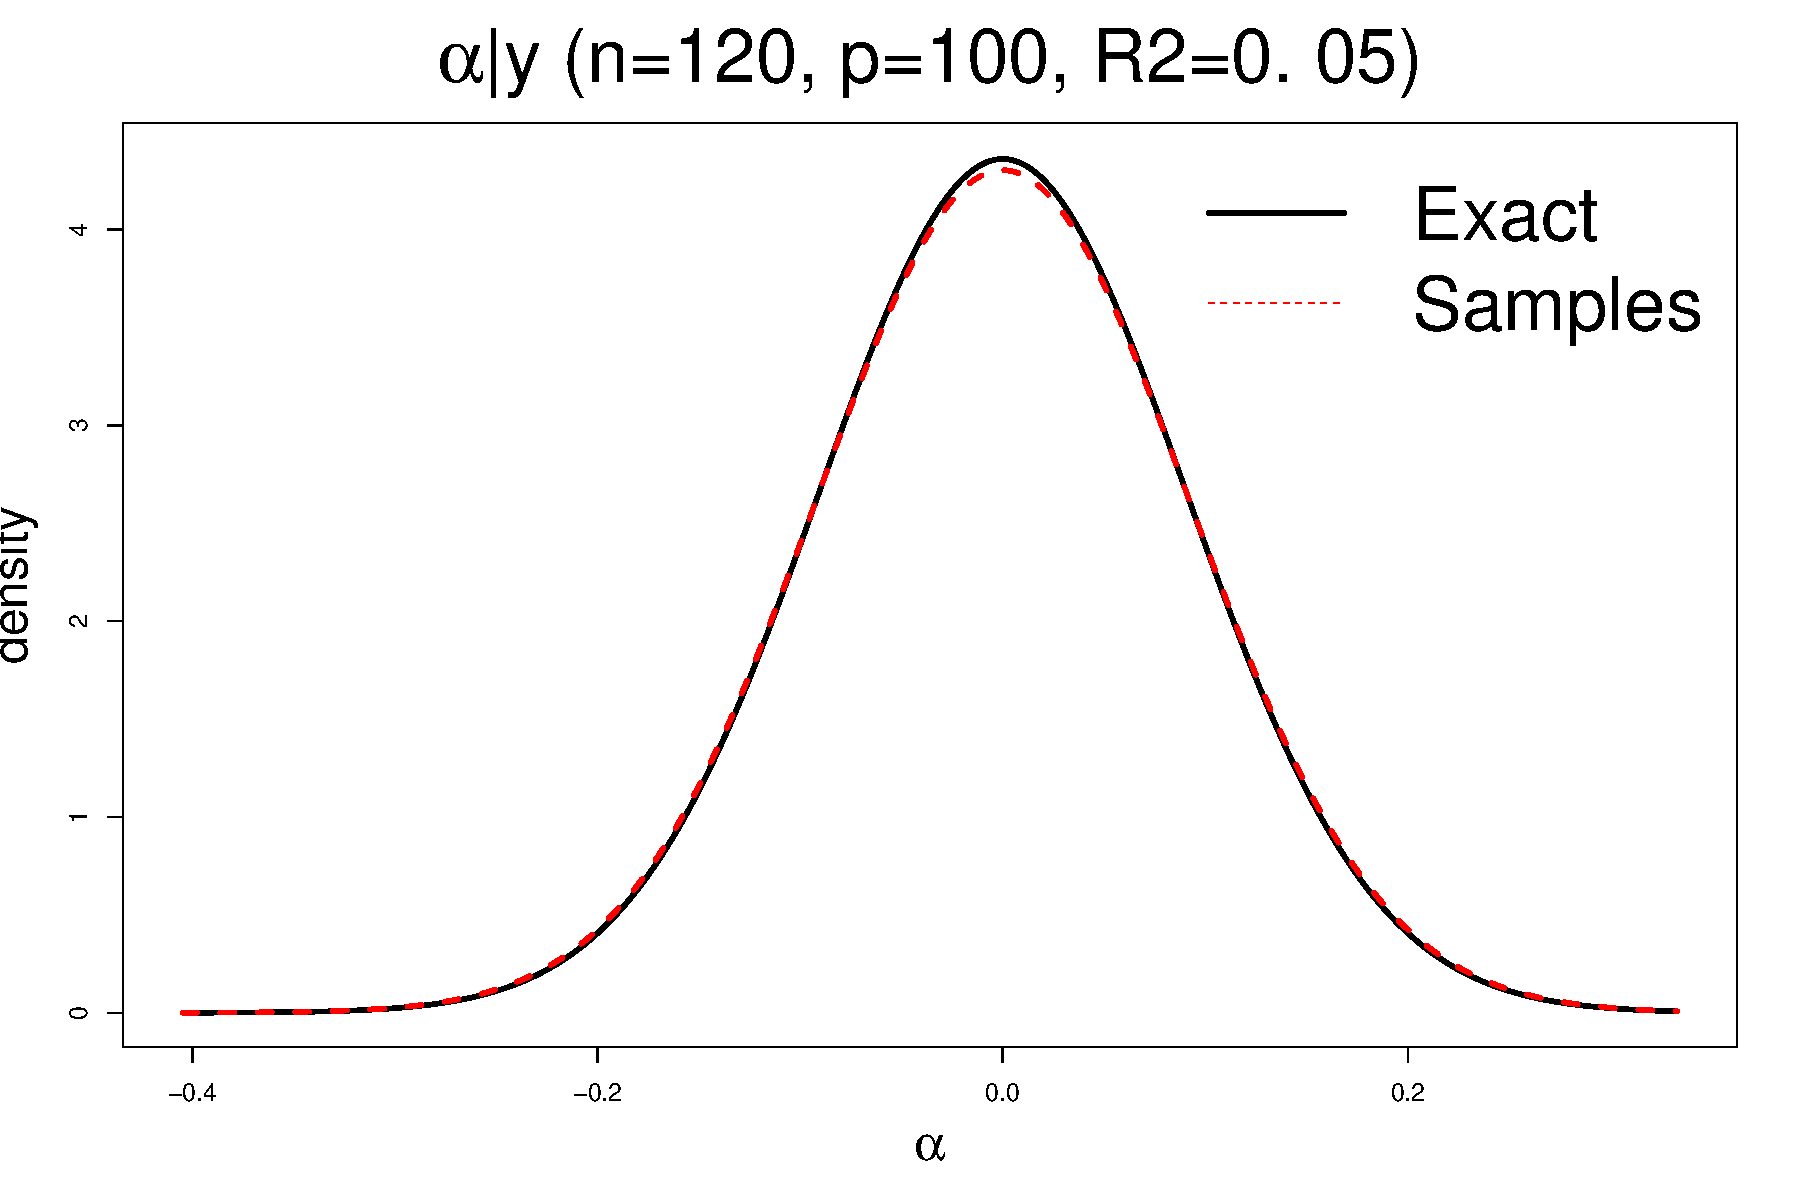
\includegraphics[width=.5\textwidth]{alphaGivenY.pdf} &
				% \caption{$\alpha | \vy$}
				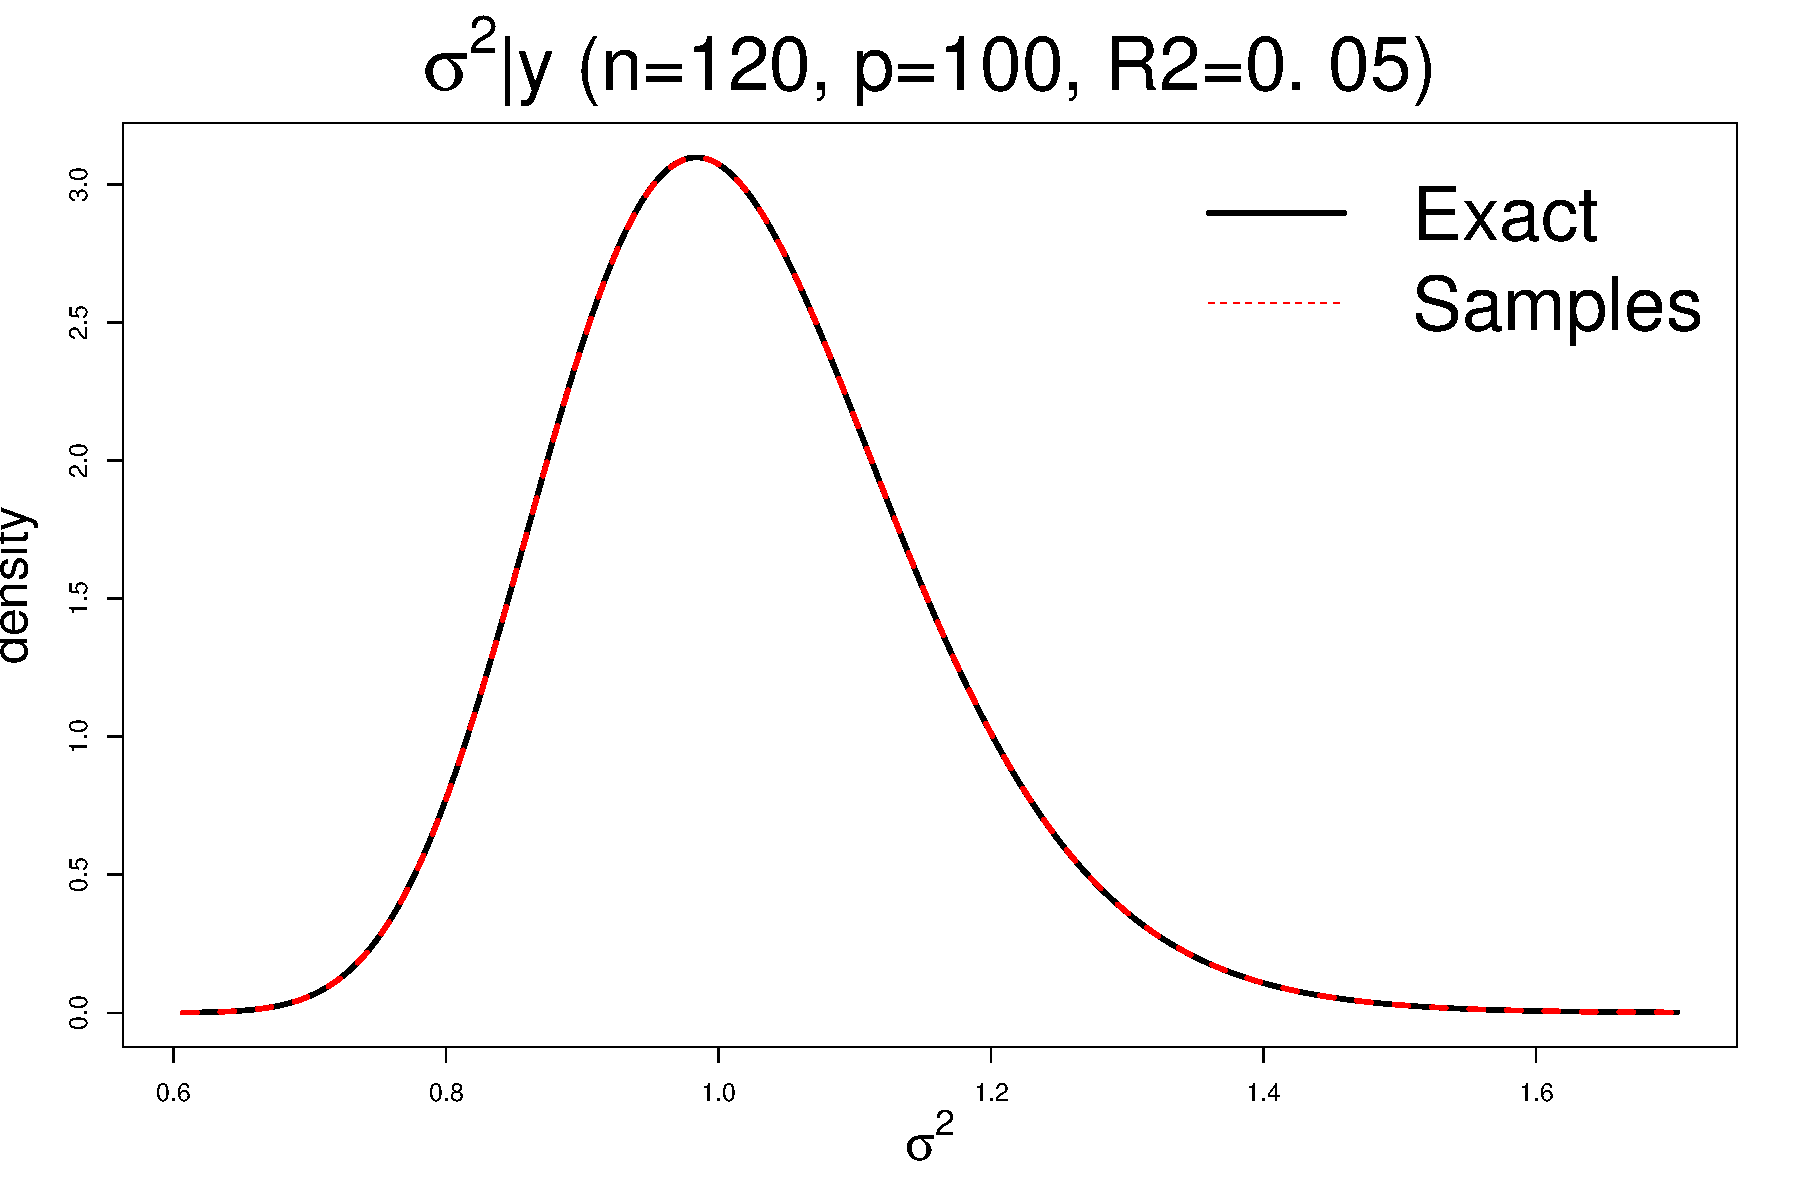
\includegraphics[width=.5\textwidth]{sigma2GivenY.pdf}
			\end{array}$
		\end{center}
	\end{figure}
\end{frame}

\note{We checked that our exact expressions were correct by checking them against a Rao-Blackwellisation sampling
			scheme that we developed, which can be considered the gold standard.
			We found that they matched very closely for a range of parameter settings.

			The inexactness of the Monte Carlo densities came about because of sampling error. Our expressions are much faster to evaluate and more accurate.

			In the event that we run into numerical problems, we can fall back on the MC scheme.}

\begin{frame}
	\frametitle{Application: Hitters data}
	\begin{figure}
		\caption{Example model fit to the Hitters data}
		\includegraphics[scale=.33]{BetaHitters.pdf}
	\end{figure}
\end{frame}

\note{We applied our model fitting software to the Hitters data set, and found that our
			first and second moments fit well.}

\begin{frame}
	\frametitle{Conclusion/Future work}
	\begin{itemize}
		\item We found exact expressions for the posterior distributions which were accurate, fast and numerically
					stable.
		\item These expressions are for a single model. When using these expressions for many models, we are able
					to perform Bayesian model averaging quickly.
		\item This is just one part of the work we're doing, which includes efficient model averaging, different
					priors on $g$ and alternatives to MCMC for model selection.
		\item This work will be made available in an \texttt{R} package on CRAN.
	\end{itemize}
\end{frame}

\begin{frame}
	\frametitle{References / Contact details}
	Thank you for your attention. Are there any questions?
	\begin{itemize}
		\item Mark Greenaway
		\item Email: \texttt{markg@maths.usyd.edu.au}
		\item Twitter: \texttt{@certifiedwaif}
		\item GitHub: \texttt{github.com/certifiedwaif}
	\end{itemize}

	\small
	\bibliographystyle{elsarticle-harv}
	\bibliography{../references_mendeley}
\end{frame}

\note{Thank you for your attention! Any questions?}

\end{document}
